\chapter{Appendices}\label{chap: append}
\section{String message priority test}\label{chap: append-string-priority}
%
%priority tests
\begin{figure}[htb]
    \centering
    \begin{subfigure}[b]{0.99\textwidth}
    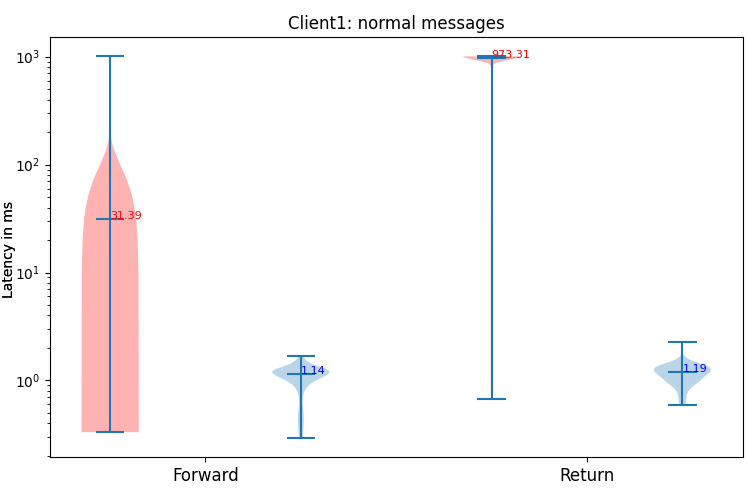
\includegraphics[width=\textwidth]{figures/appendix/priority_tests/log_violin_2clients_string_priority_client1.png}\hfill 
    \caption{} \label{fig: priority-2clients-string-1}
    \end{subfigure}
    \begin{subfigure}[b]{0.99\textwidth}
        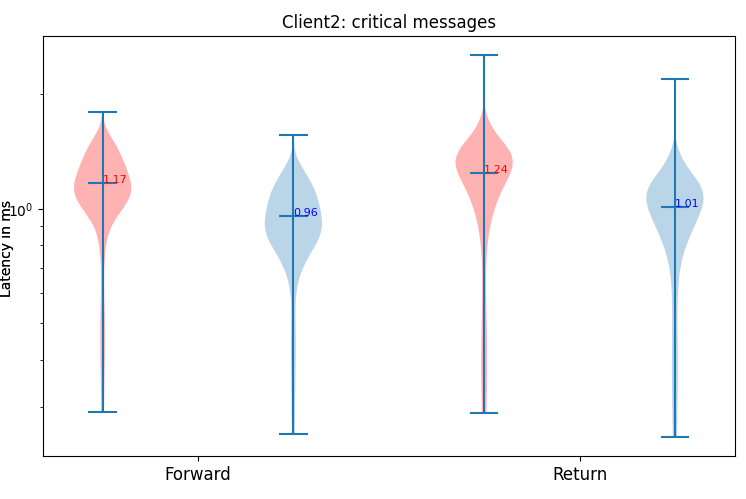
\includegraphics[width=\textwidth]{figures/appendix/priority_tests/log_violin_2clients_string_priority_client2.png}\hfill 
        \caption{} \label{fig: priority-2clients-string-2}
    \end{subfigure}
    
    
    \caption{Tests for mean \gls{rtt} of forward and return prioritized string messages between 2 clients 
    and clientR for 100 times. The blue violin represents the average data transmission time and the red violin 
    respresent mean \gls{rtt}. (a) Client1 with normals messages, and (b) 
    with critical messages} \label{fig: priority-2clients-string}
\end{figure}



\begin{sidewaysfigure}[htb]
    \centering
    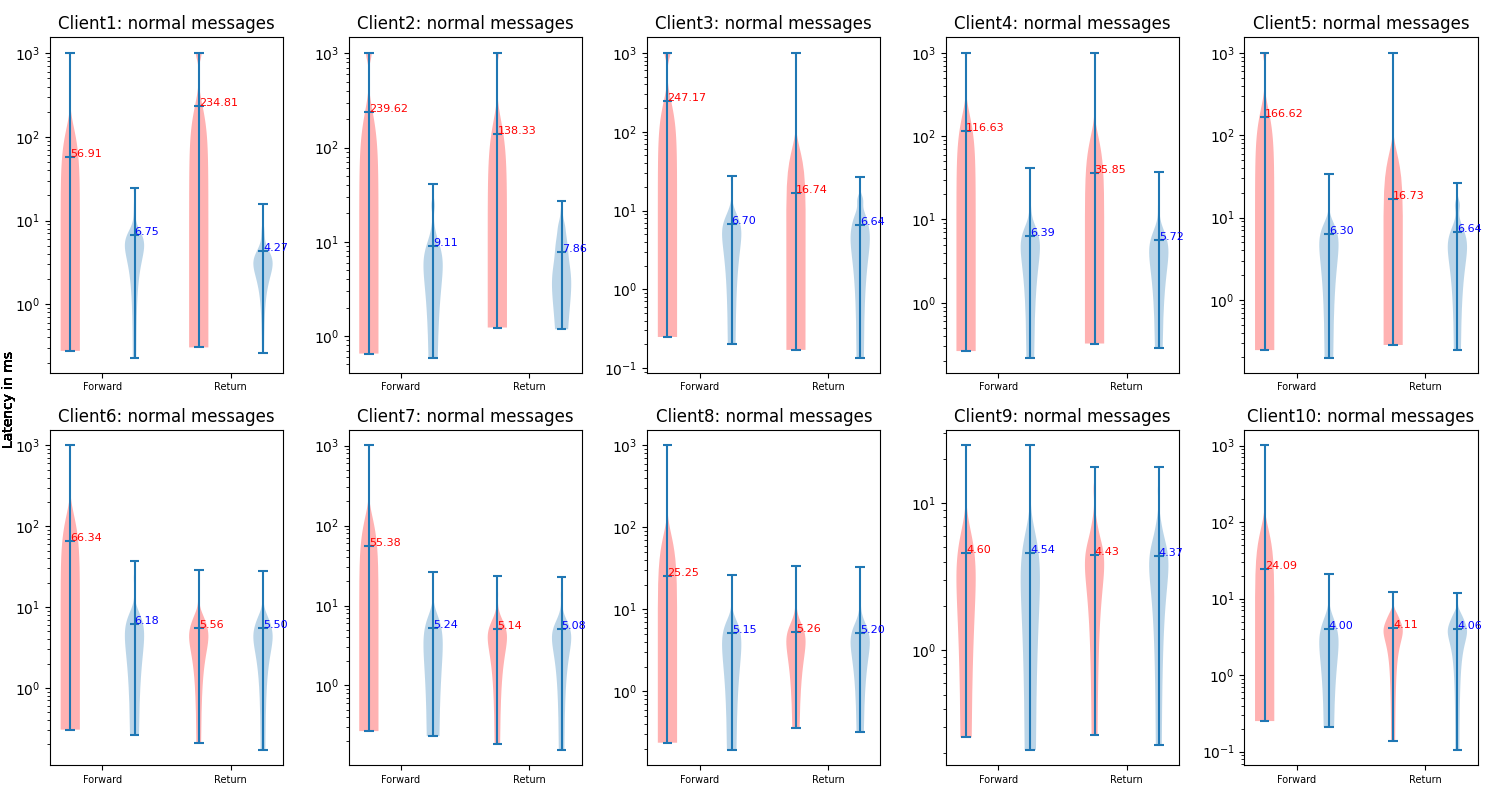
\includegraphics[width=\textheight]{figures/appendix/priority_tests/log_violin_50clients_string_figure_1.png}\hfill 
    \caption{Tests for mean \gls{rtt} of forward and return prioritized string messages between client1 to client10 
    with clientR for 100 times. The blue violin represents the average data transmission time and the red violin 
    respresent mean \gls{rtt}.} \label{fig: priority-50clients-string-a}
\end{sidewaysfigure}

\begin{sidewaysfigure}[htb]
    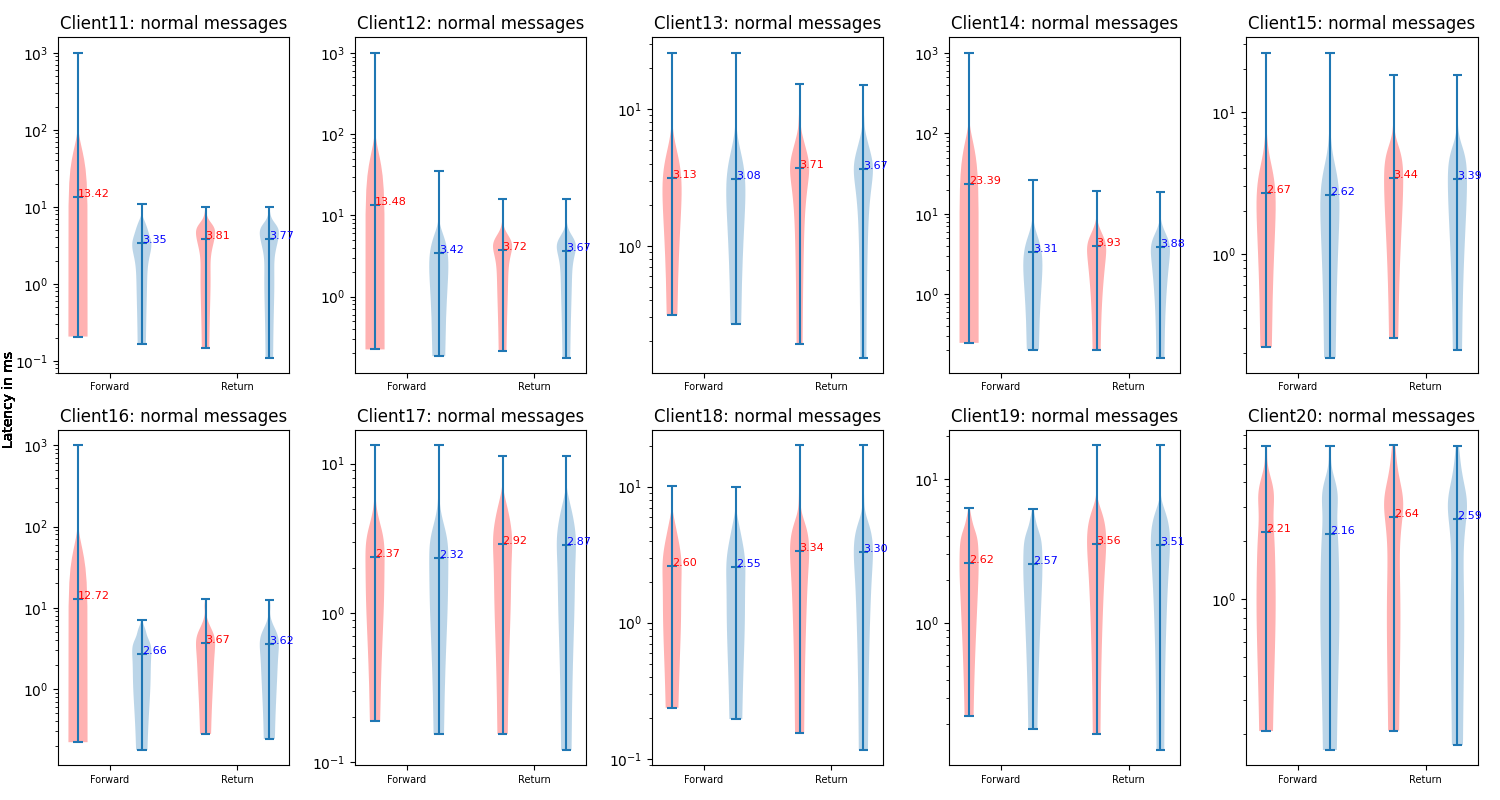
\includegraphics[width=\textheight]{figures/appendix/priority_tests/log_violin_50clients_string_figure_2.png}\hfill 
    \caption{Tests for mean \gls{rtt} of forward and return prioritized string messages between client11 to client20 
    with clientR for 100 times. The blue violin represents the average data transmission time and the red violin 
    respresent mean \gls{rtt}.} \label{fig: priority-50clients-string-b}
\end{sidewaysfigure}

\begin{sidewaysfigure}[htb]
    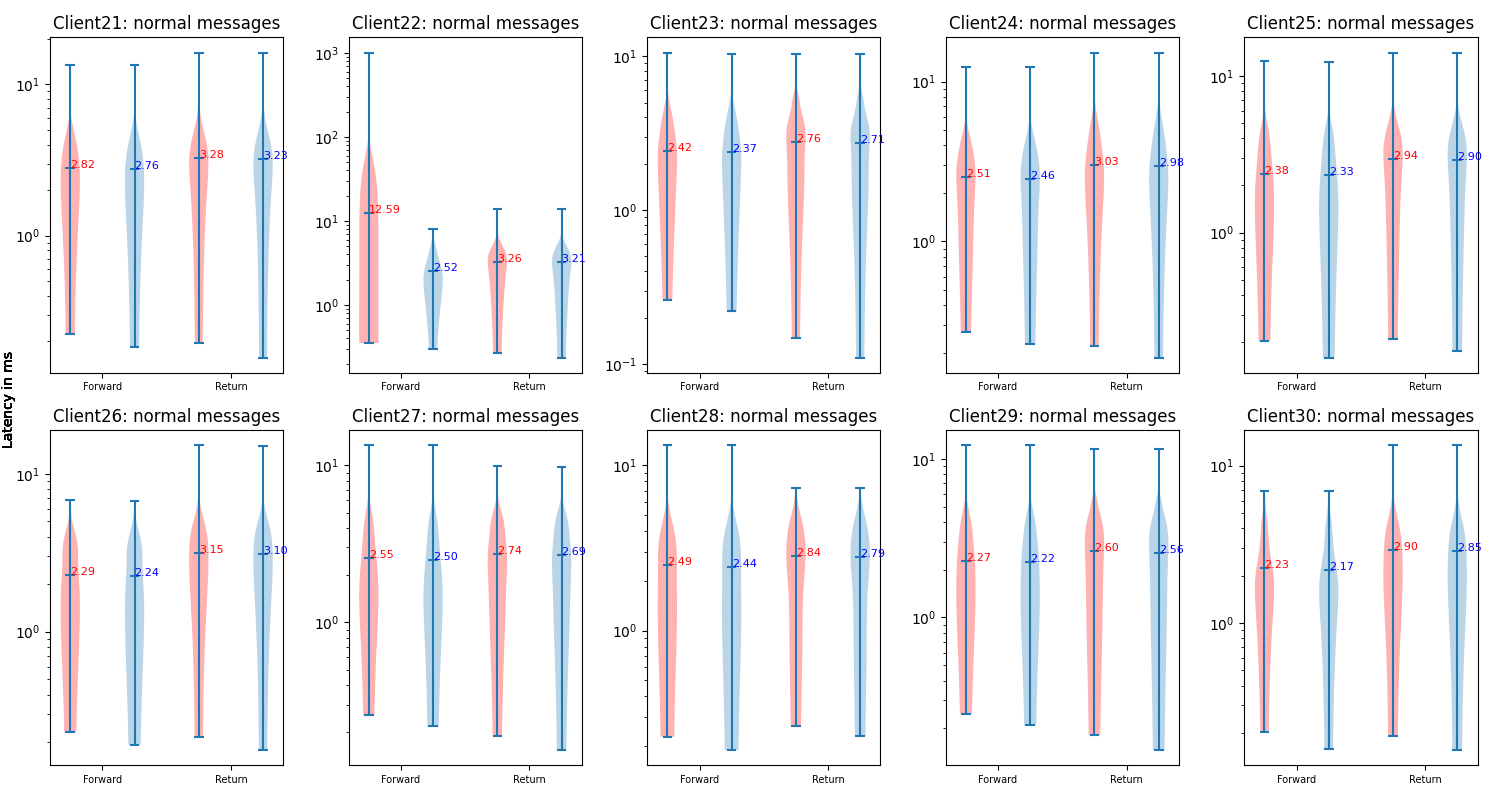
\includegraphics[width=\textheight]{figures/appendix/priority_tests/log_violin_50clients_string_figure_3.png}\hfill 
    \caption{Tests for mean \gls{rtt} of forward and return prioritized string messages between client21 to client30 
    with clientR for 100 times. The blue violin represents the average data transmission time and the red violin 
    respresent mean \gls{rtt}.} \label{fig: priority-50clients-string-c}
\end{sidewaysfigure}

\begin{sidewaysfigure}[htb]
    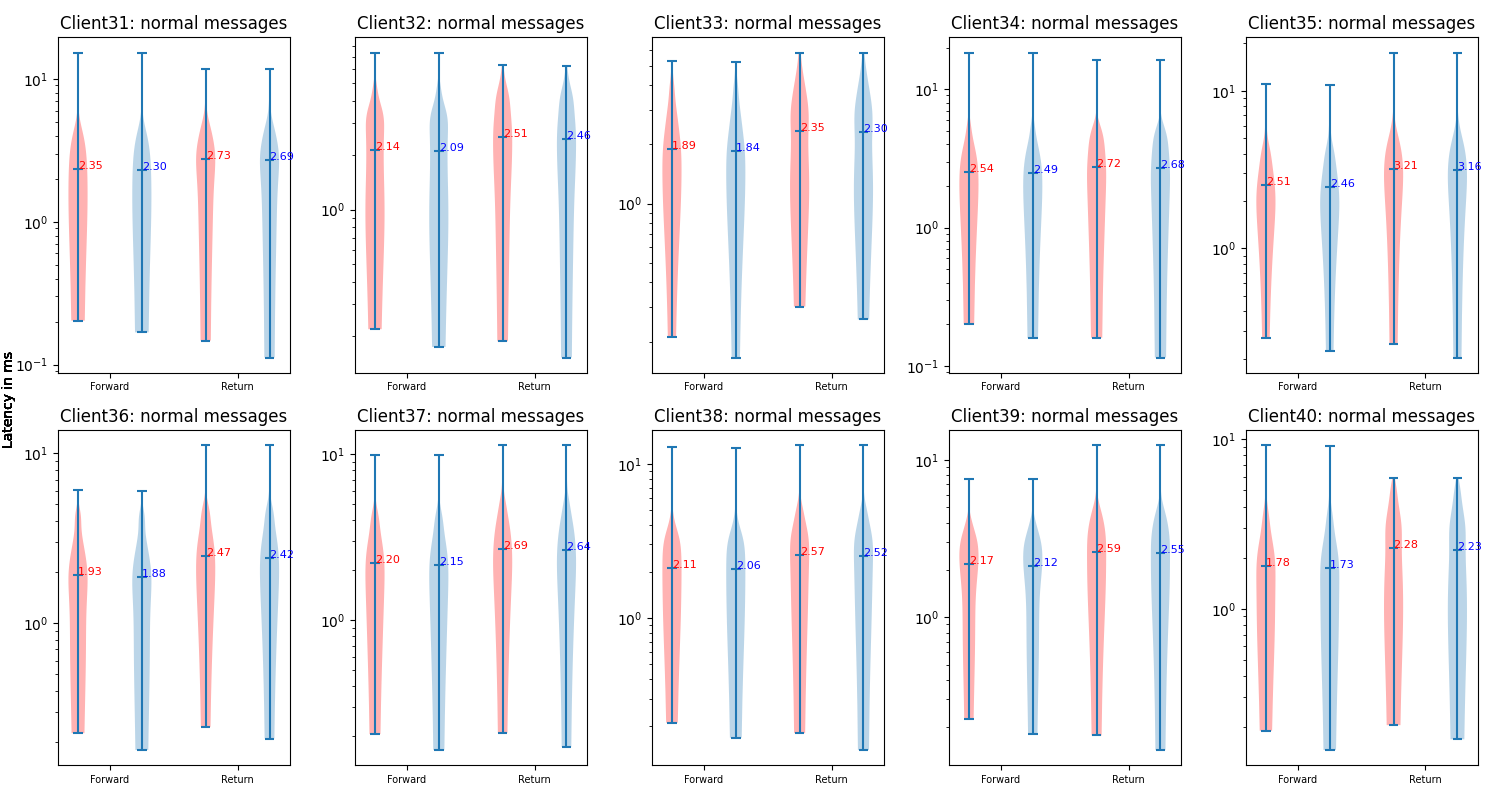
\includegraphics[width=\textheight]{figures/appendix/priority_tests/log_violin_50clients_string_figure_4.png}\hfill 
    \caption{Tests for mean \gls{rtt} of forward and return prioritized string messages between client31 to client40 
    with clientR for 100 times. The blue violin represents the average data transmission time and the red violin 
    respresent mean \gls{rtt}.} \label{fig: priority-50clients-string-d}
\end{sidewaysfigure}

\begin{sidewaysfigure}[htb]
    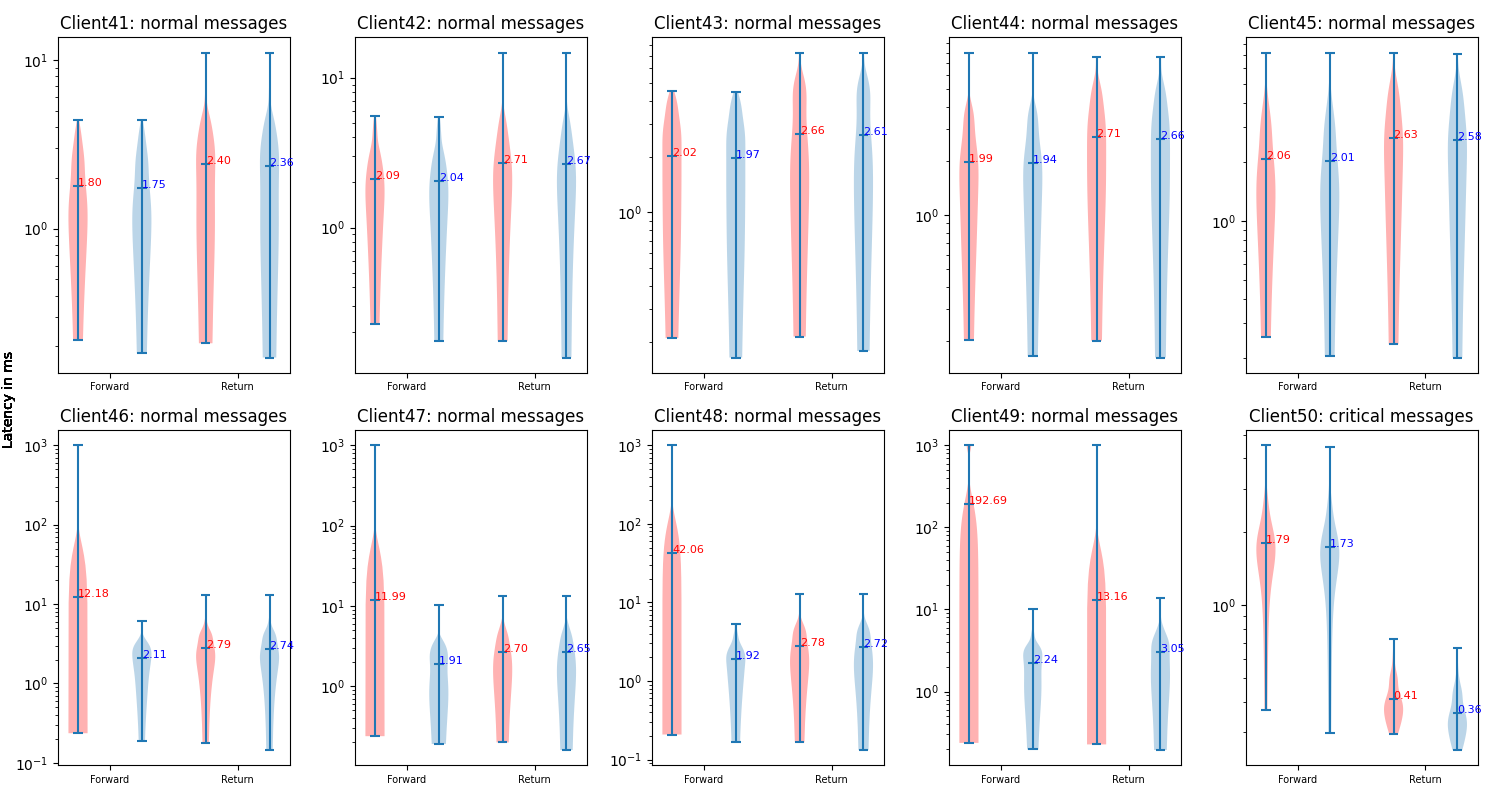
\includegraphics[width=\textheight]{figures/appendix/priority_tests/log_violin_50clients_string_figure_5.png}\hfill 
    \caption{Tests for mean \gls{rtt} of forward and return prioritized string messages between client41 to client50 
    with clientR for 100 times. The blue violin represents the average data transmission time and the red violin 
    respresent mean \gls{rtt}.} \label{fig: priority-50clients-string-e}
\end{sidewaysfigure}



\section{Image message priority test}\label{chap: append-image-priority}


\begin{figure}[htb]
    \centering
    \begin{subfigure}[b]{0.99\textwidth}
    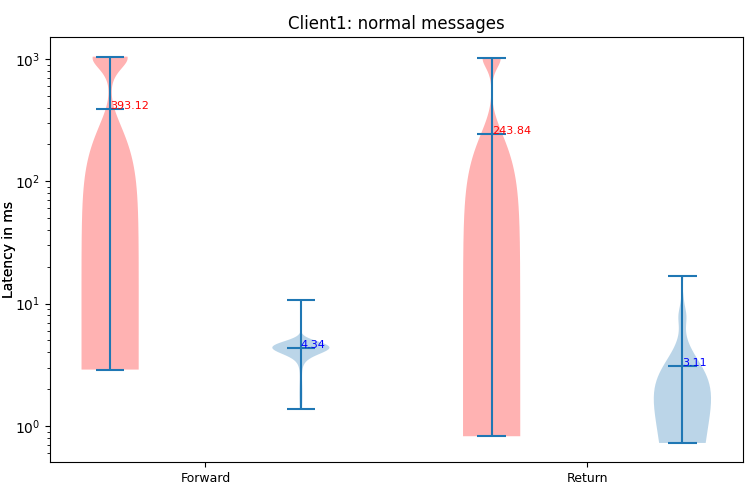
\includegraphics[width=\textwidth]{figures/appendix/priority_tests/log_violin_2clients_image_priority_client1.png}\hfill 
    \caption{} \label{fig: priority-2clients-image-1}
    \end{subfigure}
    \begin{subfigure}[b]{0.99\textwidth}
        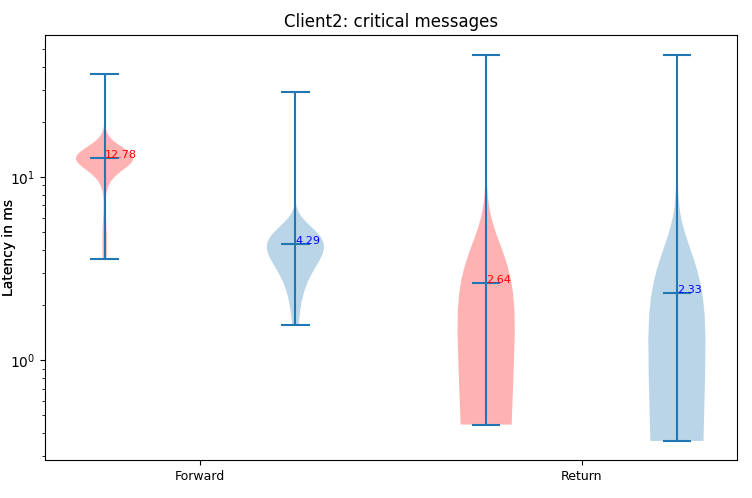
\includegraphics[width=\textwidth]{figures/appendix/priority_tests/log_violin_2clients_image_priority_client2.png}\hfill 
        \caption{} \label{fig: priority-2clients-image-2}
    \end{subfigure}
    
    
    \caption{Tests for mean \gls{rtt} of forward and return prioritized image messages between 2 clients 
    and clientR for 100 times. The blue violin represents the average data transmission time and the red violin 
    respresent mean \gls{rtt}. (a) Client1 with normals messages, and (b) 
    with critical messages} \label{fig: priority-2clients-image}
\end{figure}



\begin{sidewaysfigure}[htb]
    \centering
    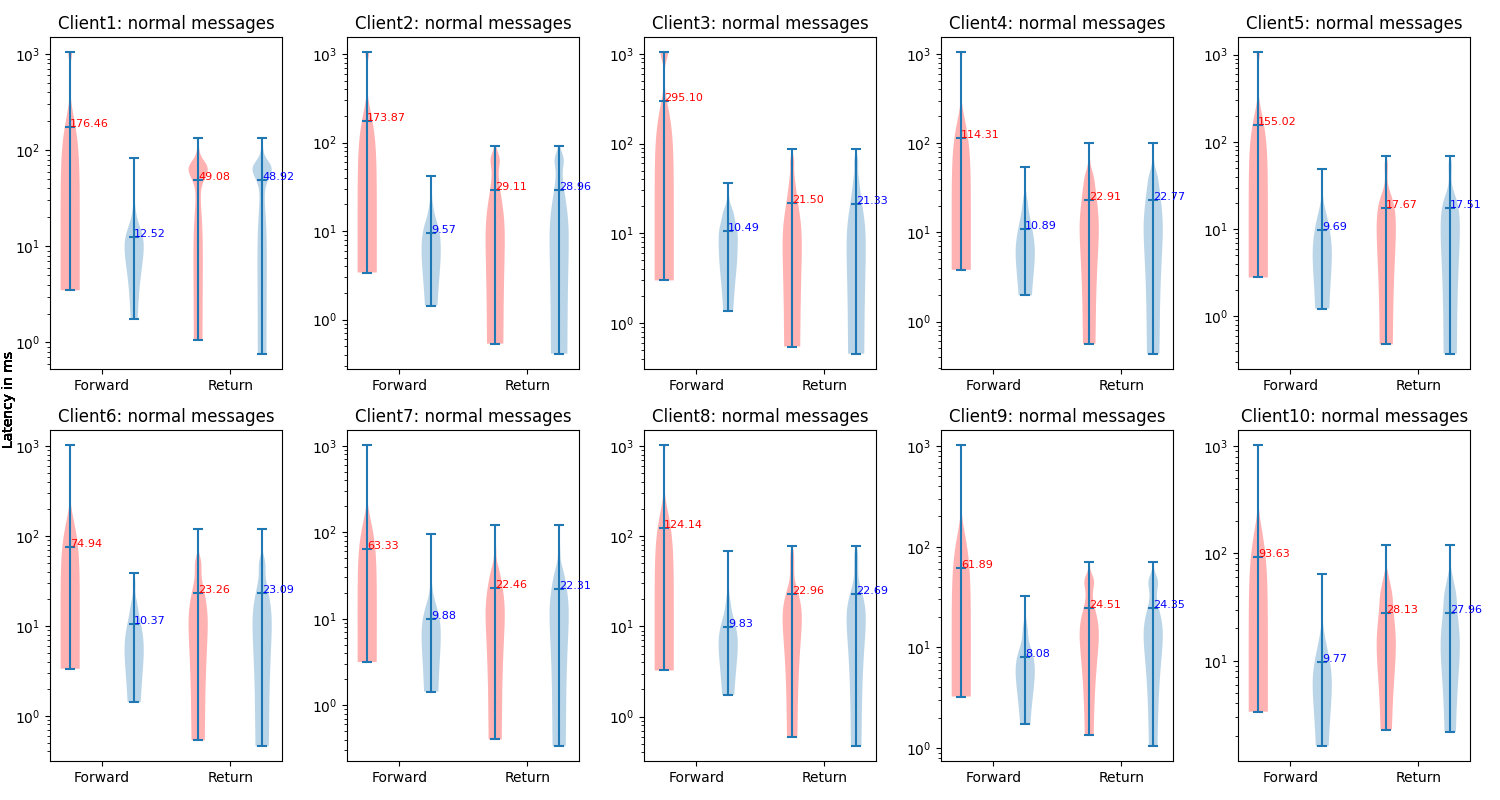
\includegraphics[width=\textheight]{figures/appendix/priority_tests/log_violin_50clients_image_figure_1.png}\hfill 
    \caption{Tests for mean \gls{rtt} of forward and return prioritized image messages between client1 to client10 
    with clientR for 100 times. The blue violin represents the average data transmission time and the red violin 
    respresent mean \gls{rtt}.} \label{fig: priority-50clients-image-a}
\end{sidewaysfigure}

\begin{sidewaysfigure}[htb]
    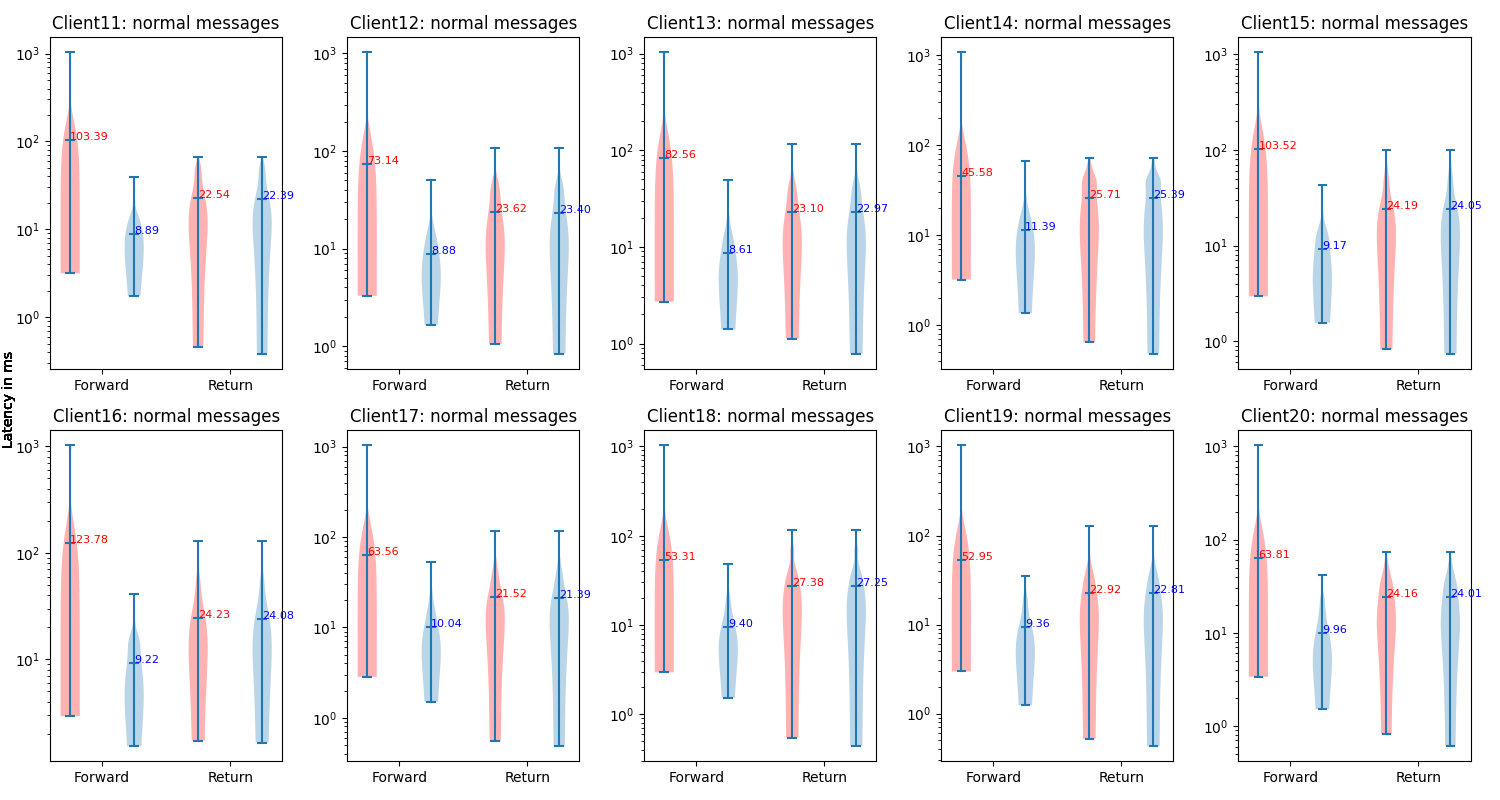
\includegraphics[width=\textheight]{figures/appendix/priority_tests/log_violin_50clients_image_figure_2.png}\hfill 
    \caption{Tests for mean \gls{rtt} of forward and return prioritized image messages between client11 to client20 
    with clientR for 100 times. The blue violin represents the average data transmission time and the red violin 
    respresent mean \gls{rtt}.} \label{fig: priority-50clients-image-b}
\end{sidewaysfigure}

\begin{sidewaysfigure}[htb]
    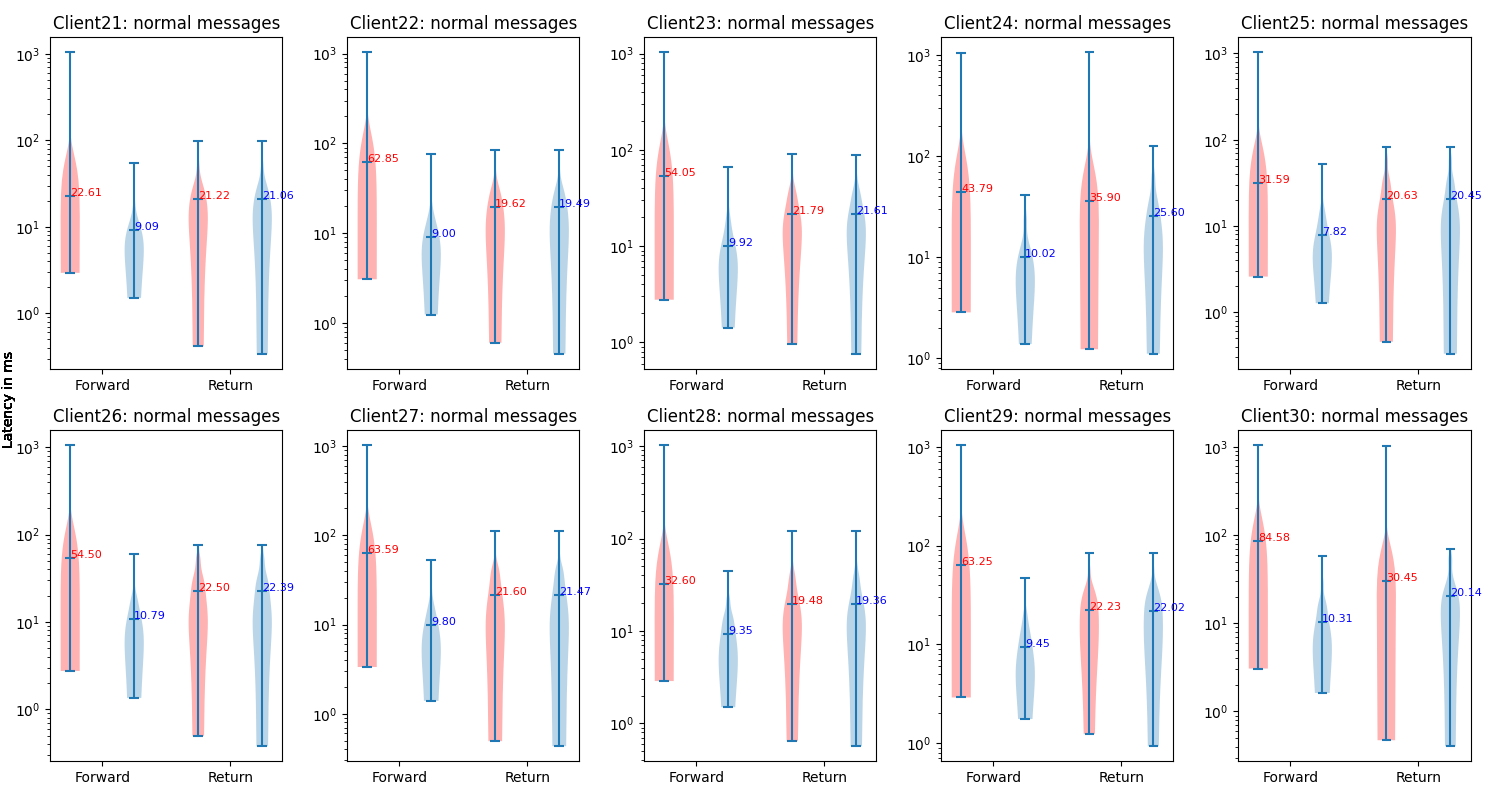
\includegraphics[width=\textheight]{figures/appendix/priority_tests/log_violin_50clients_image_figure_3.png}\hfill 
    \caption{Tests for mean \gls{rtt} of forward and return prioritized image messages between client21 to client30 
    with clientR for 100 times. The blue violin represents the average data transmission time and the red violin 
    respresent mean \gls{rtt}.} \label{fig: priority-50clients-image-c}
\end{sidewaysfigure}

\begin{sidewaysfigure}[htb]
    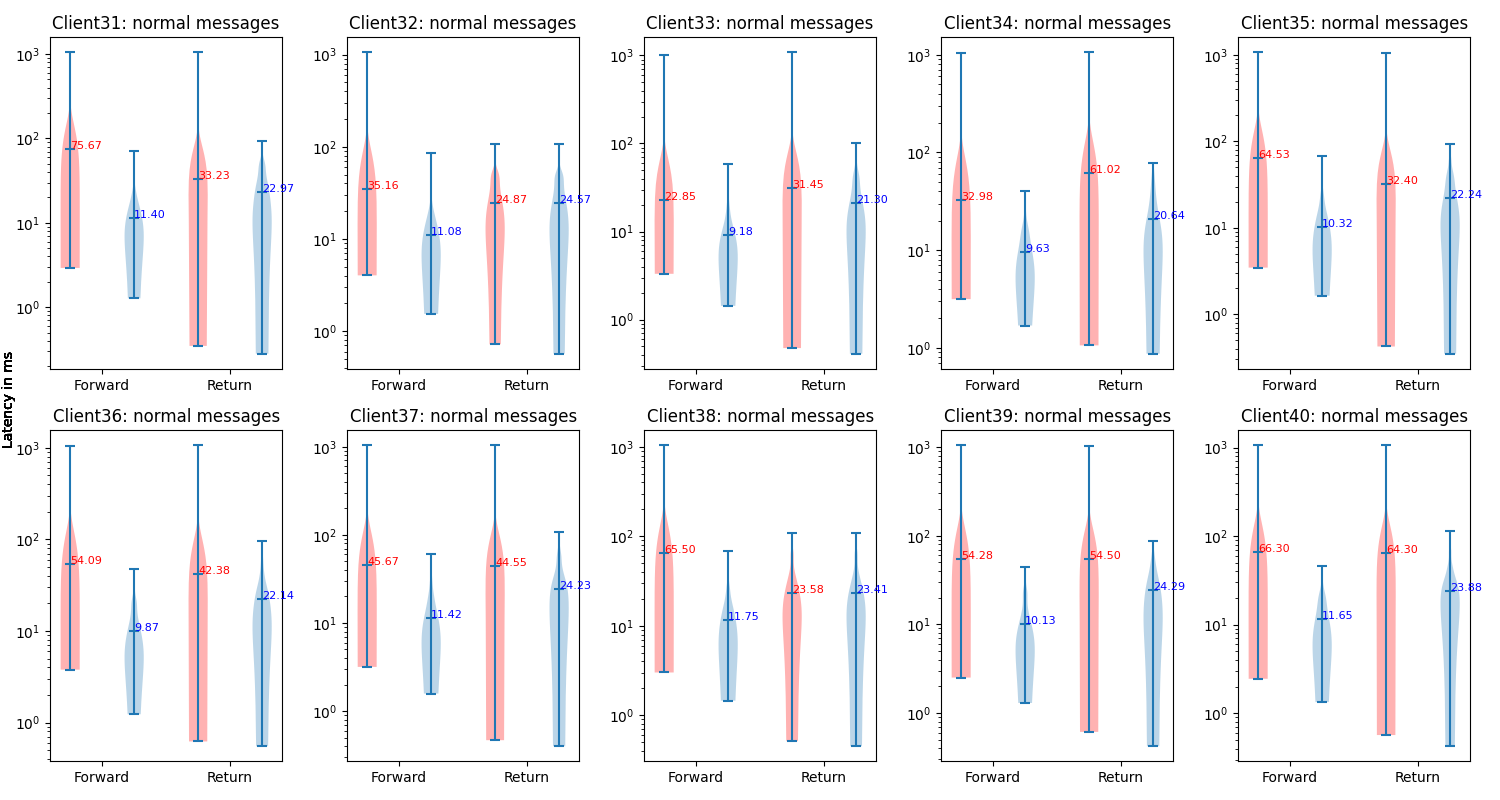
\includegraphics[width=\textheight]{figures/appendix/priority_tests/log_violin_50clients_image_figure_4.png}\hfill 
    \caption{Tests for mean \gls{rtt} of forward and return prioritized image messages between client31 to client40 
    with clientR for 100 times. The blue violin represents the average data transmission time and the red violin 
    respresent mean \gls{rtt}.} \label{fig: priority-50clients-image-d}
\end{sidewaysfigure}

\begin{sidewaysfigure}[htb]
    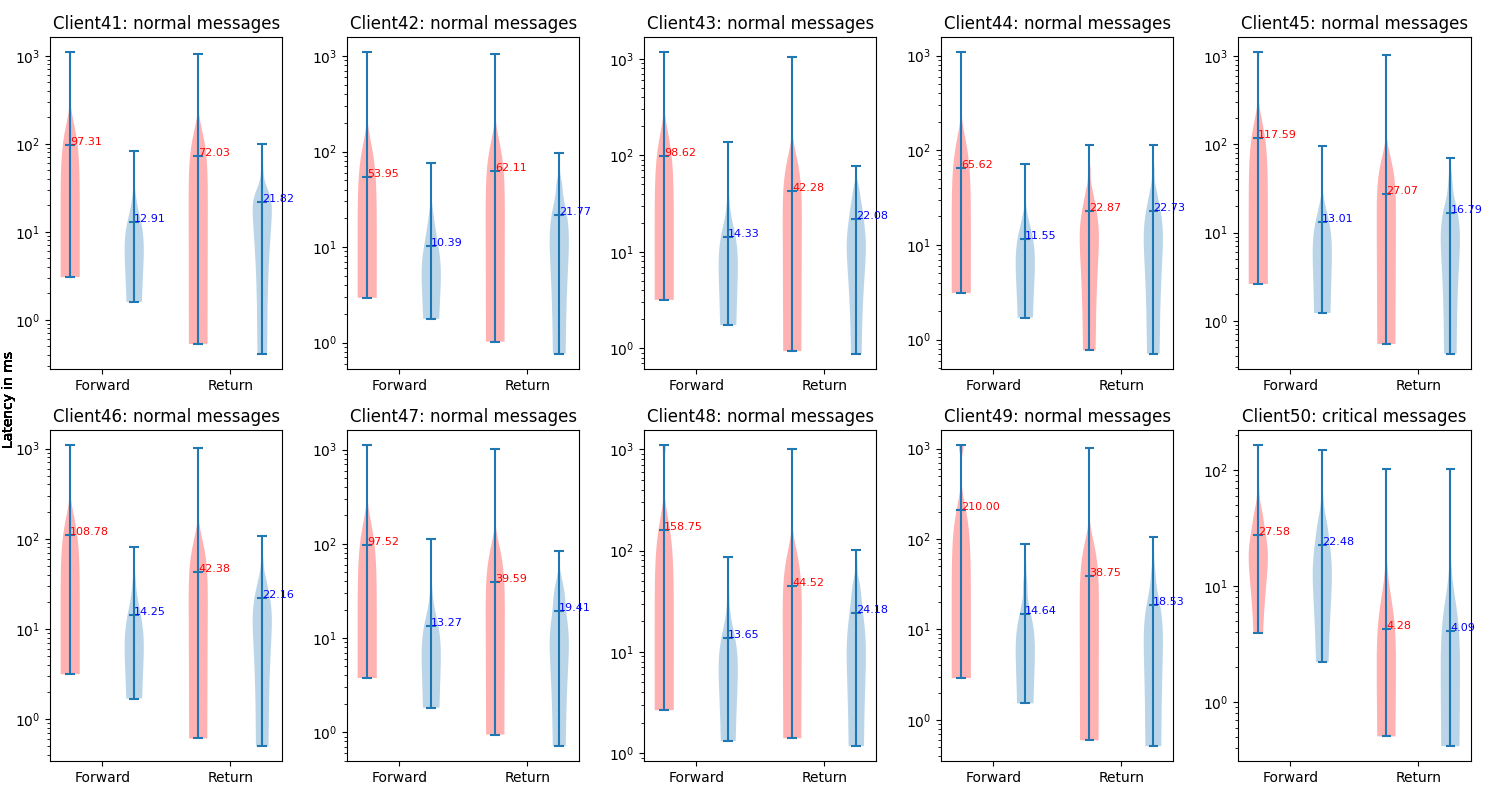
\includegraphics[width=\textheight]{figures/appendix/priority_tests/log_violin_50clients_image_figure_5.png}\hfill 
    \caption{Tests for mean \gls{rtt} of forward and return prioritized image messages between client41 to client50 
    with clientR for 100 times. The blue violin represents the average data transmission time and the red violin 
    respresent mean \gls{rtt}.} \label{fig: priority-50clients-image-e}
\end{sidewaysfigure}




%use cases
\section{Use case based test}\label{chap: append-UC}

\begin{figure}[htb]
    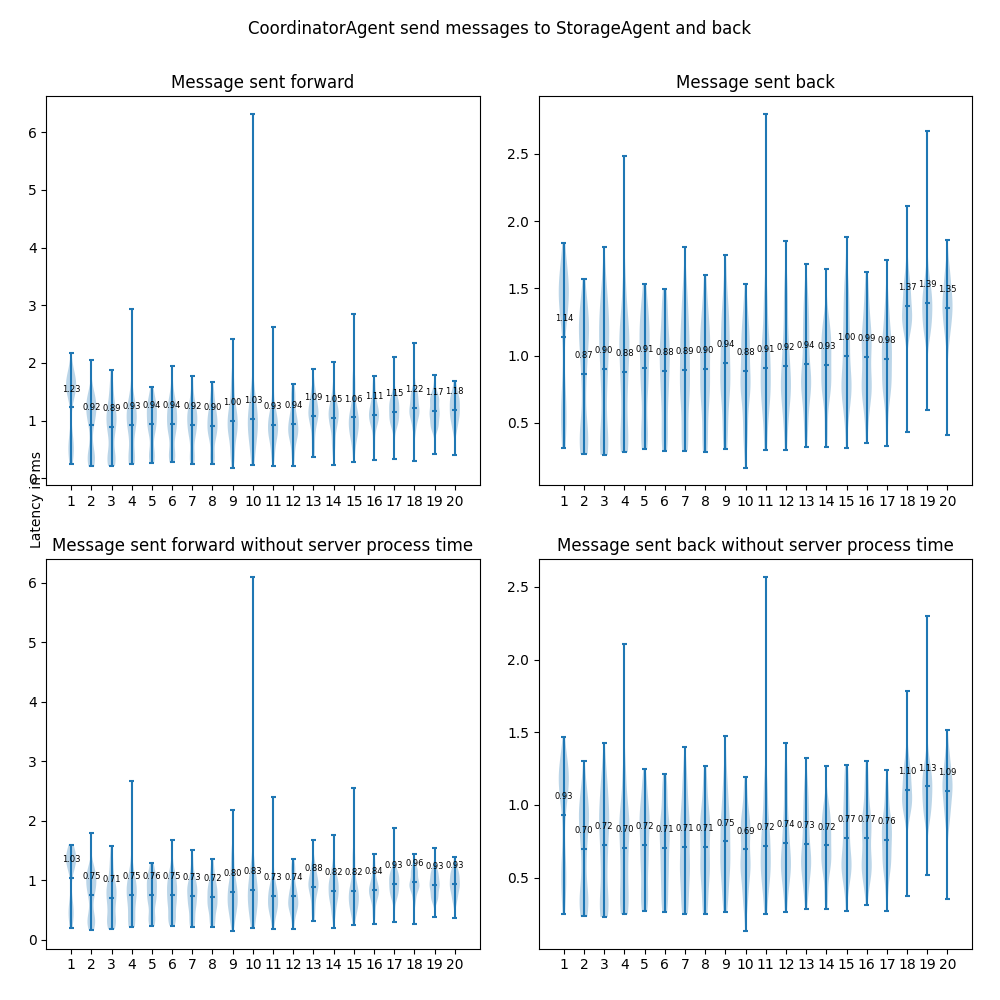
\includegraphics[width=\textwidth]{figures/appendix/usecase/violin_CoordinatorAgent_to_StorageAgent.png}
    \centering
    \caption{Test to measure \gls{rtt} and transmission time between \gls{cda} and 
    StorageAgent for 100 times. The number in x-axis respresents the 
    corresonding messages. \protect\ref{firstfootnote}}
    \label{fig: violin-CDA-ST}
\end{figure}


\begin{figure}[htb]
    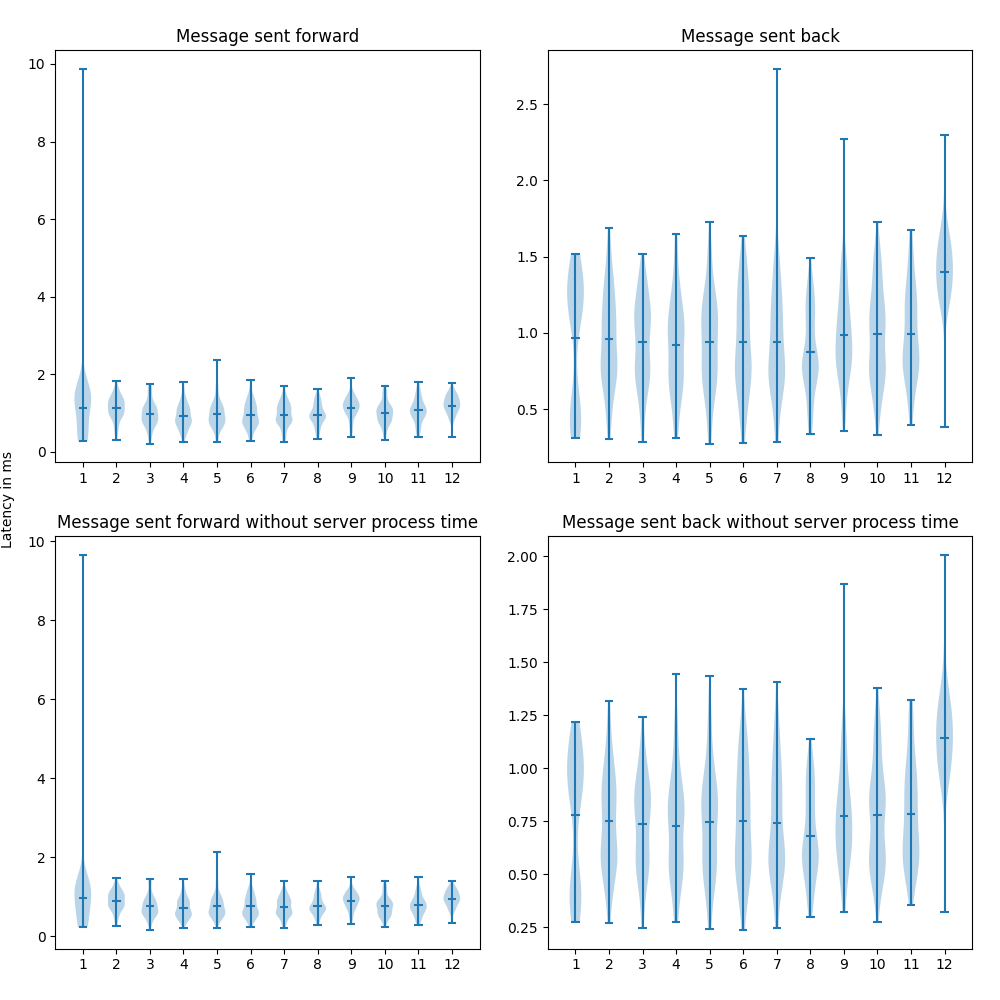
\includegraphics[width=\textwidth]{figures/appendix/usecase/violin_CoordinatorAgent_to_WiringAgent.png}
    \centering
    \caption{Test to measure \gls{rtt} and transmission time between \gls{cda} and 
    WiringAgent for 100 times. The number in x-axis respresents the 
    corresonding messages. \protect\ref{firstfootnote}}
    \label{fig: violin-CDA-WI}
\end{figure}


\begin{figure}[htb]
    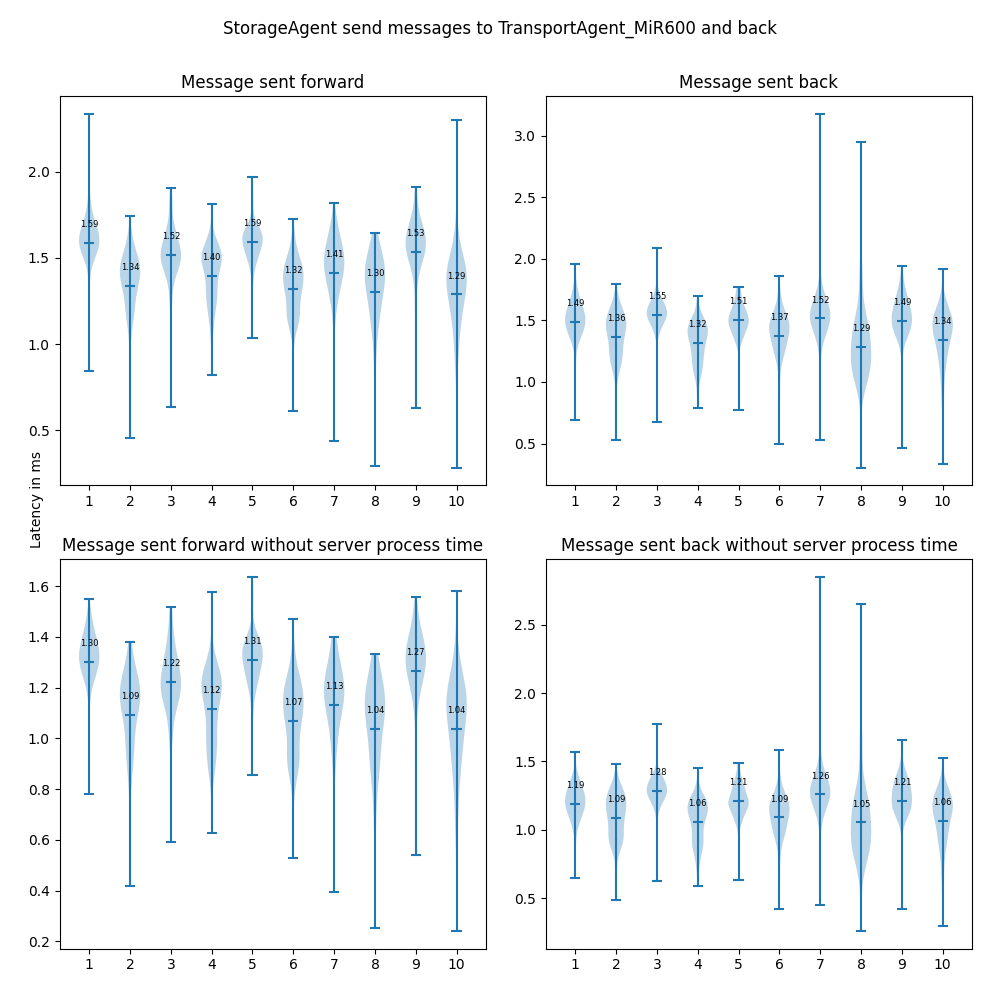
\includegraphics[width=\textwidth]{figures/appendix/usecase/violin_StorageAgent_to_TransportAgent_MiR600.png}
    \centering
    \caption{Test to measure \gls{rtt} and transmission time between StorageAgent and 
    TransportAgent\_MiR600 for 100 times. The number in x-axis respresents the 
    corresonding messages. \protect\ref{firstfootnote}}
    \label{fig: violin-ST-T600}
\end{figure}

\begin{figure}[htb]
    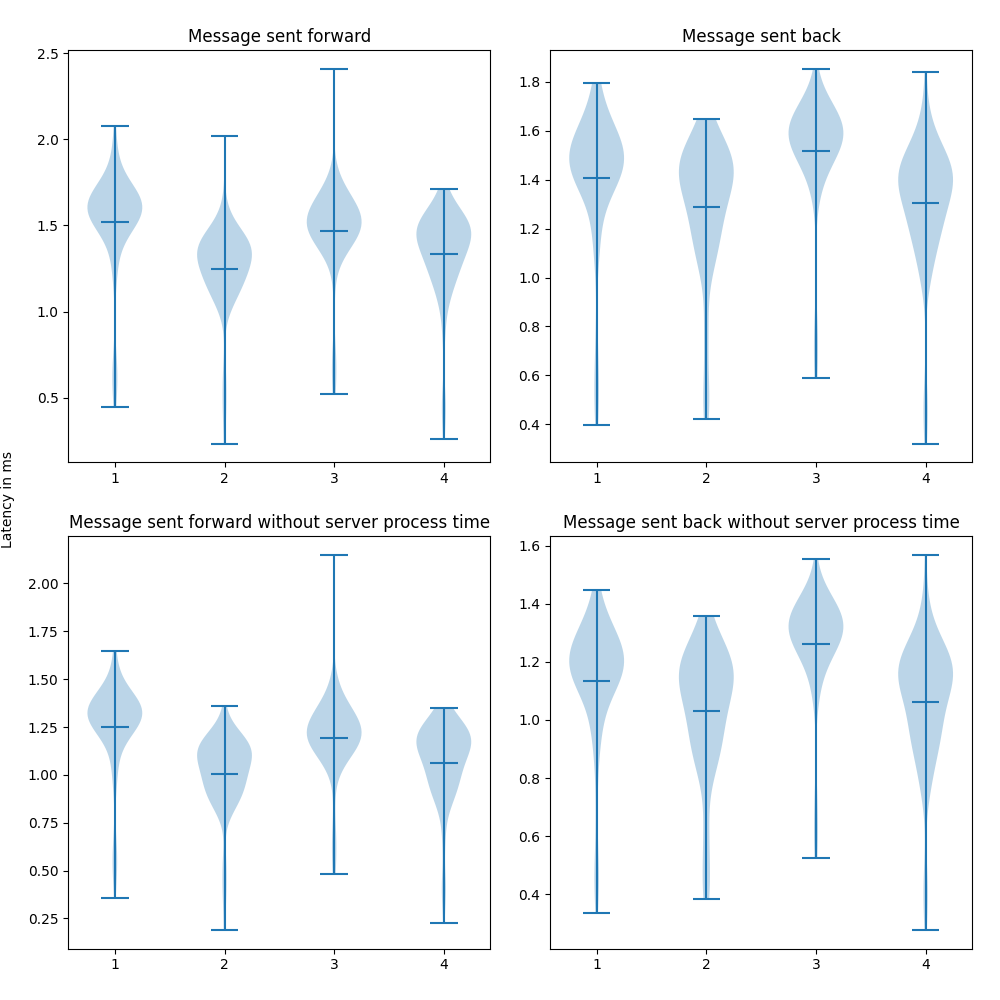
\includegraphics[width=\textwidth]{figures/appendix/usecase/violin_TransportAgent_MiR600_to_WiringAgent.png}
    \centering
    \caption{Test to measure \gls{rtt} and transmission time between TransportAgent\_MiR600 and 
    WiringAgent for 100 times. The number in x-axis respresents the 
    corresonding messages. \protect\ref{firstfootnote}}
    \label{fig: violin-T600-WI}
\end{figure}





%DT
\section{\gls{dta} test}\label{chap: append-DTagent}
\begin{figure}[htb]
    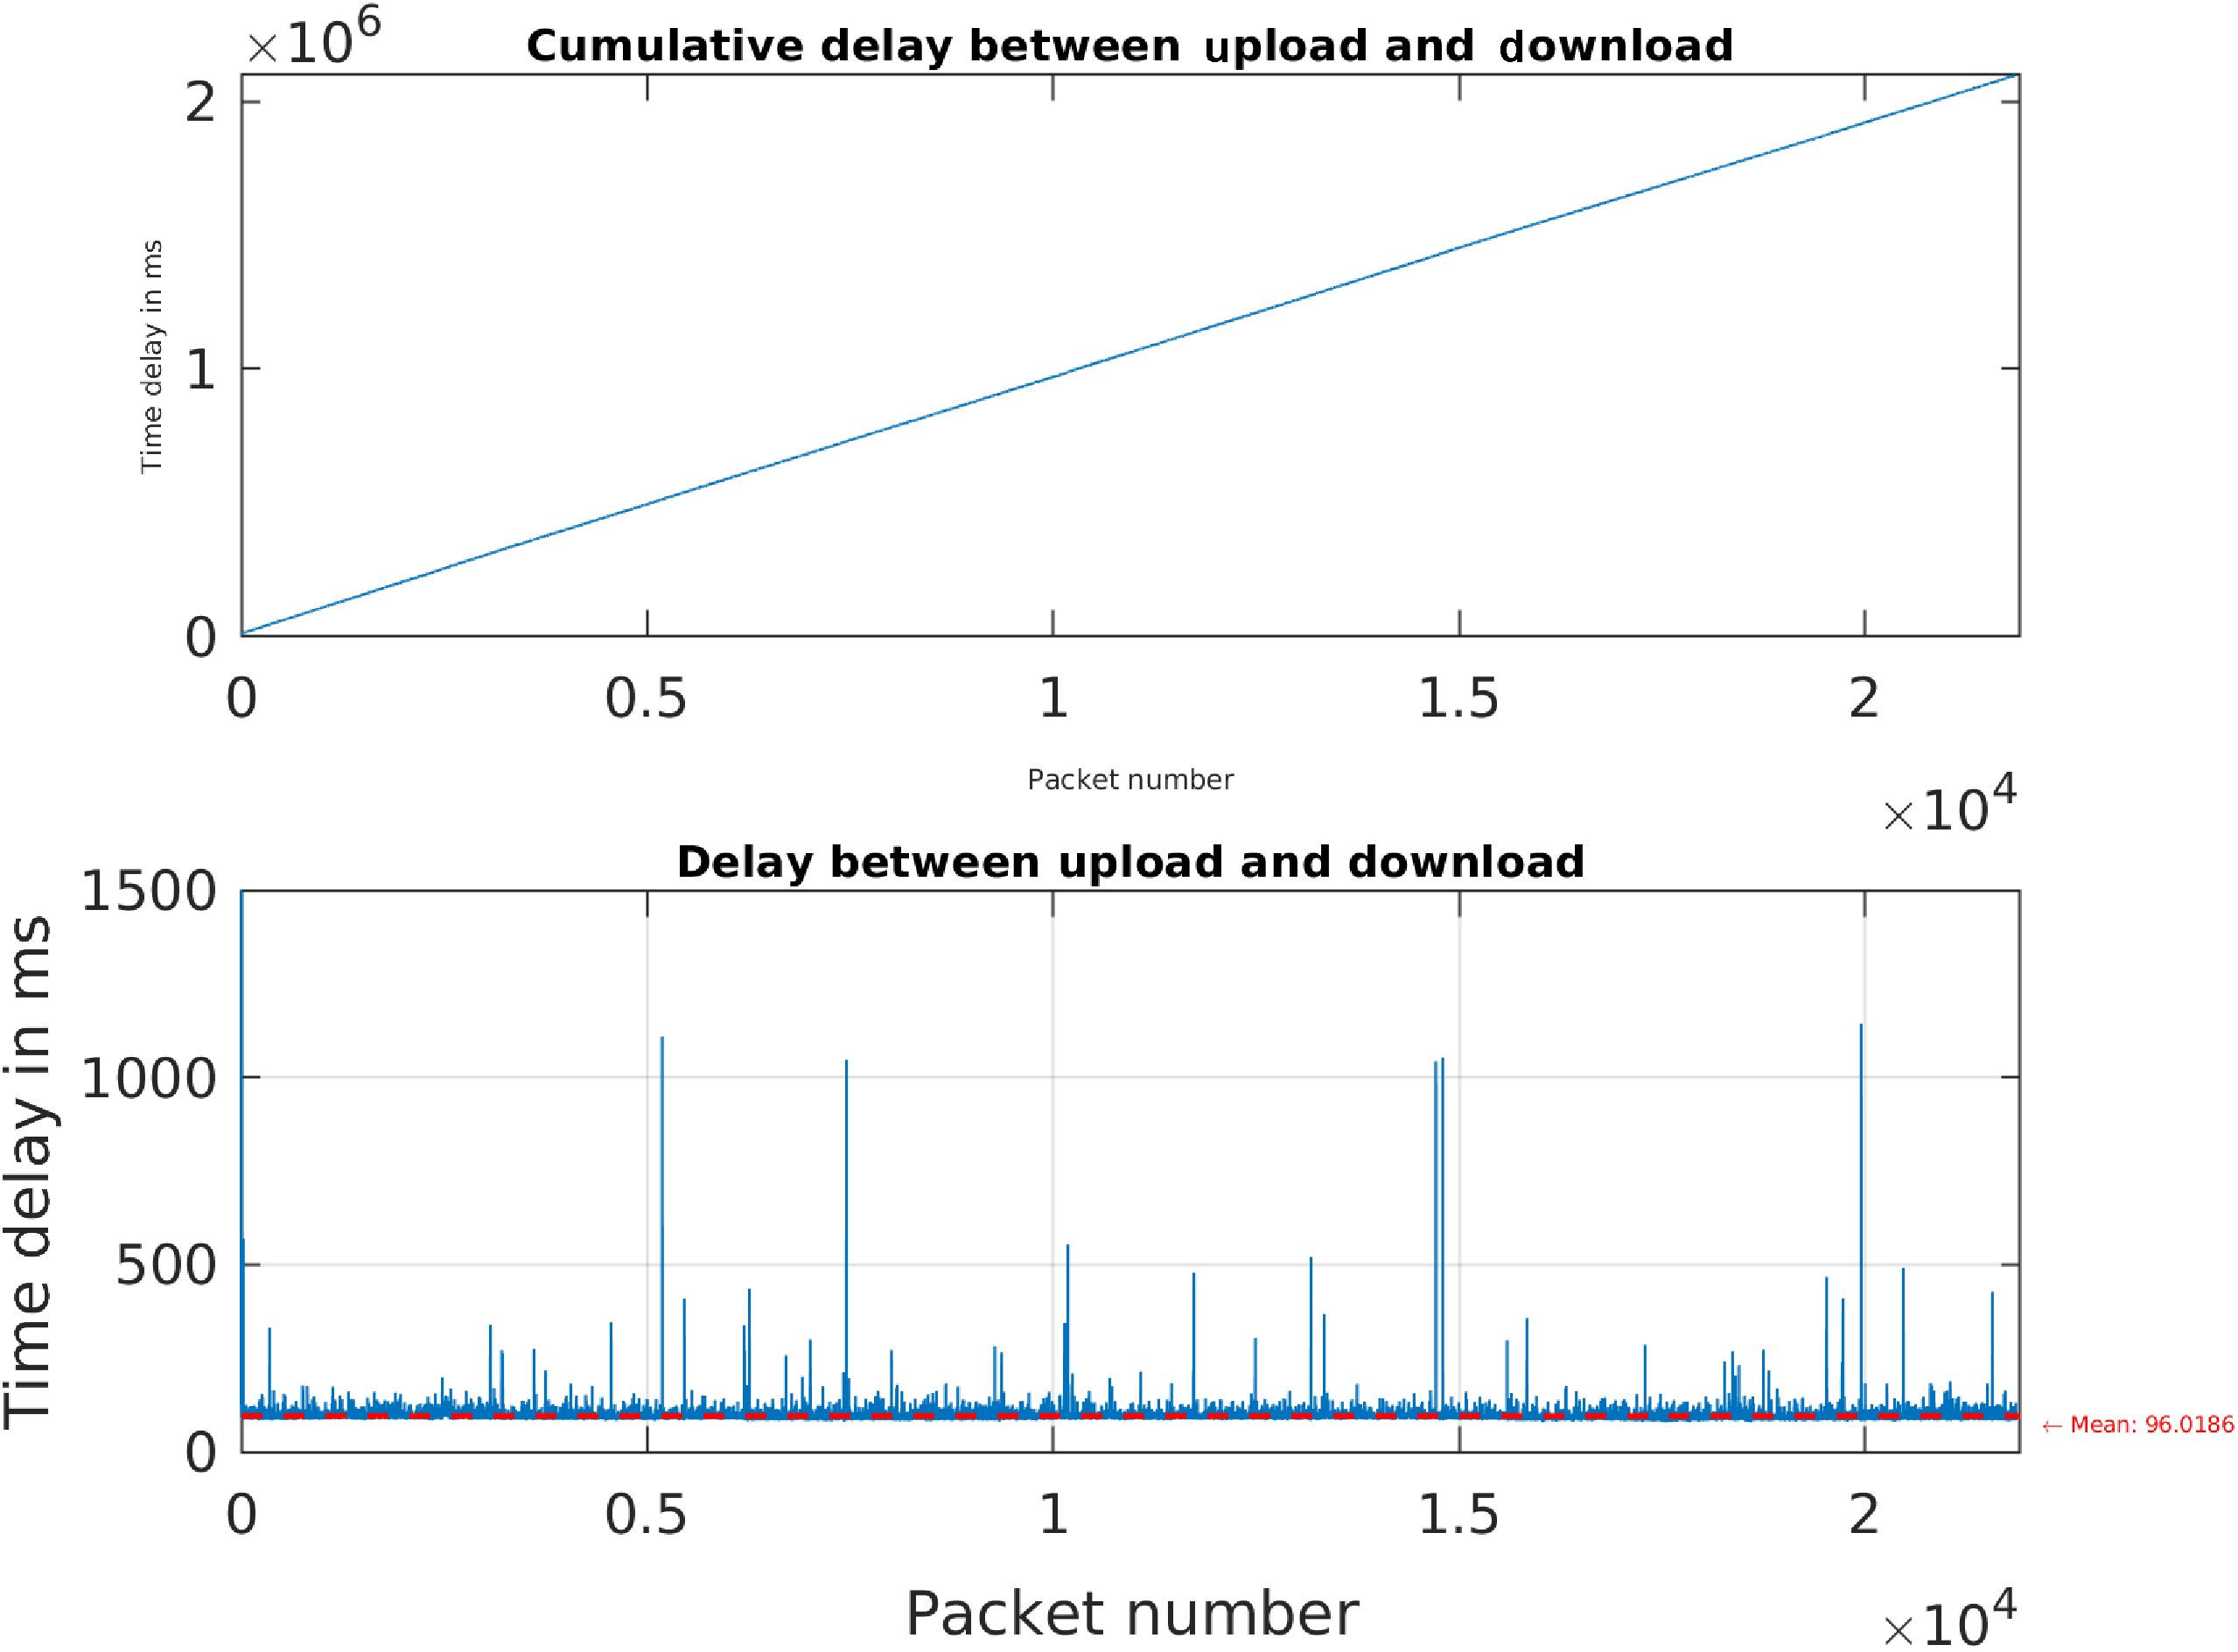
\includegraphics[width=\textwidth]{figures/appendix/DT/Delay_UploadDownloadCycleTime_Elbow.pdf}\hfill 
    \caption{Tests for \gls{rtt} of data upload and download for Elbow.} \label{fig: UD-cycle-Elbow}
\end{figure}

\begin{figure}[htb]
    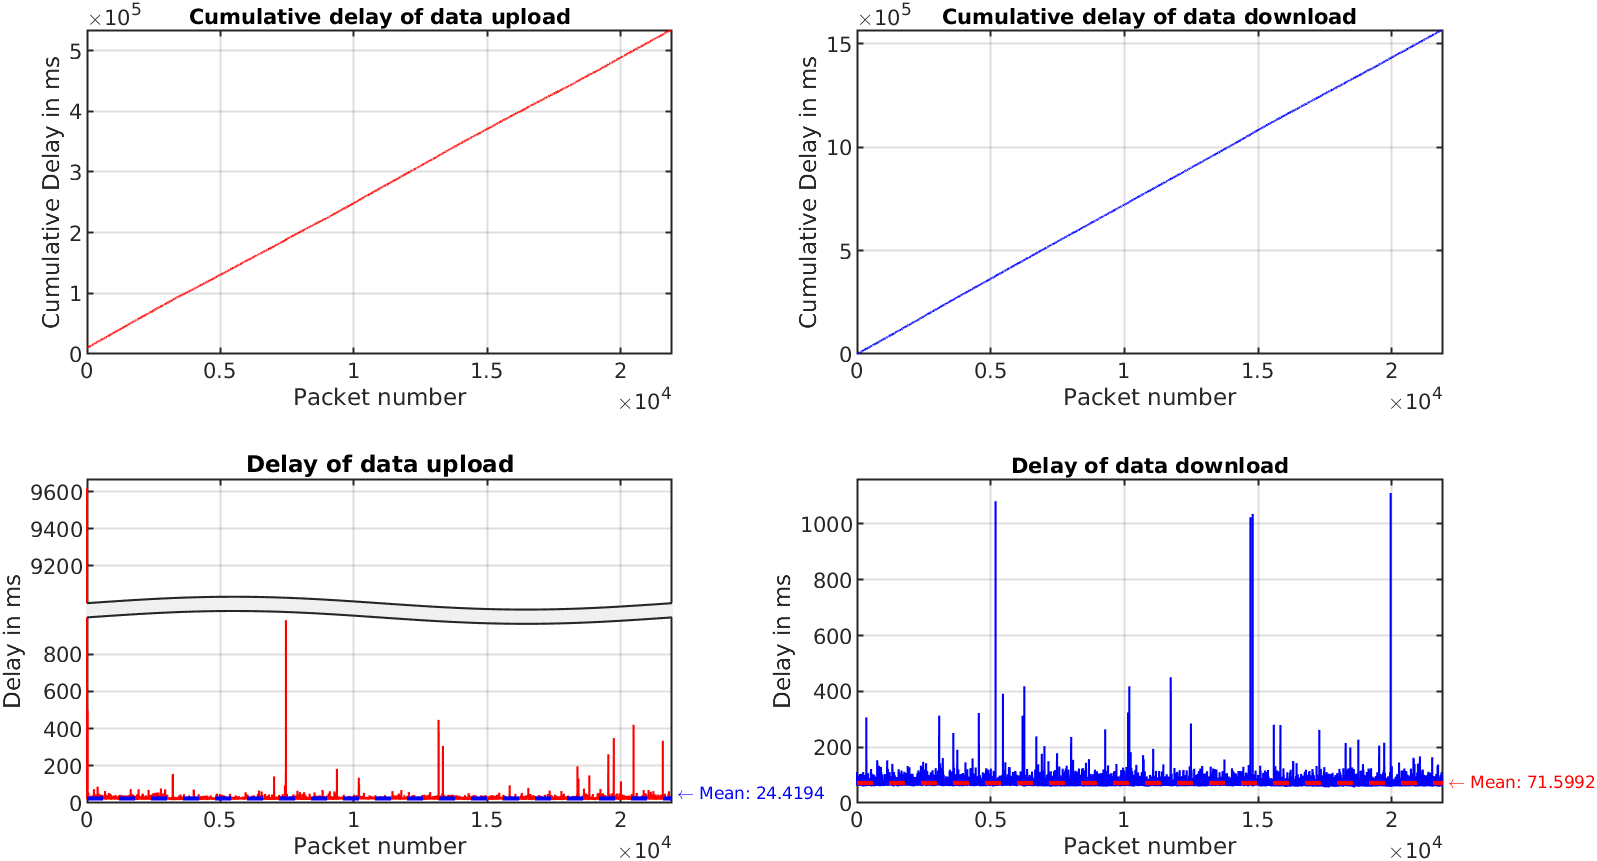
\includegraphics[width=\textwidth]{figures/appendix/DT/Delay_UploadDownload_Elbow.png}
    \centering
    \caption{Tests for delays between \gls{dta} and digital twin update of Elbow, 
    and delays for twin value download. \label{fig: UD-sep-Elbow}}
\end{figure}




%

